\documentclass[a4paper,12pt]{report}
\usepackage[utf8]{inputenc}
\usepackage[francais]{babel}
\usepackage{fancyhdr}
\usepackage{graphicx}
\usepackage{tikz}
\usetikzlibrary{calc}
\usepackage{listings}
\usepackage{xcolor}
\definecolor{grey}{rgb}{0.9,0.9,0.9}
\usepackage{titlesec}
\usepackage{verbatim}
\usepackage{listings}
\usepackage{textcomp}
\usepackage{hyperref}
\usepackage{amssymb}
\usepackage{amsmath}
\usepackage{longtable}
\usepackage{colortbl}
\usepackage{float}
\usepackage{caption}
\usepackage{subfig}


\frenchbsetup{StandardLists=true}
\newcommand{\marge}{18mm}
\usepackage[left=\marge,right=\marge,top=\marge,bottom=\marge]{geometry}
\pagestyle{fancy}
\setlength{\headheight}{14pt}
\chead{
  \textbf{Binôme :} Douaille Erwan \& François Rémy
  \hspace{2em}
  \textbf{Groupe :} M1 Info RDF}
\renewcommand{\headrulewidth}{1pt}
\linespread{1}
\setlength{\columnseprule}{0.2pt}





\begin{document}


\makeatletter
\begin{titlepage}
\centering
\vspace{-10em}
{\LARGE \textbf{\textsc{Rapport de Projet RVI}}}\\
\vspace{3em}

\includegraphics[scale=0.6]{image/thalassa.png}\\
\vspace{3em}
{\LARGE \textsc{Projet Thalassa: simulation de plongée sous-marine}}\\

\vspace{8em}
Par\\
\vspace{1em}
{\LARGE \@author}\\

\vspace{2em}



\begin{tikzpicture}[remember picture,overlay]

\node [below left,xshift=-1cm, yshift=4cm] at (current page.south east){
\includegraphics[scale=0.6]{image/ustl1.png}};

\end{tikzpicture}
\end{titlepage}
\makeatother

\sloppy

\setcounter{page}{1} 
\newpage

%%%%%%%%%%%%%%%%%%%%%%%%%%%%%%%%%%%% INTRODUCTION
%%%%%%%%%%%%%%%%%%%%%%%%%%%%%%%%%%%%%%%%%%%%%%%%%
%%%%%%%%%%%%%%%%%%%%%%%%%%%%%%%%%%%%%%%%%%%%%%%%%
\section*{Introduction}
Le but de ce TP est de montrer plusieurs méthodes de binarisation d'image. La binarisation permet d'obtenir une image de 2 couleurs, nette et plus facile à analyser. Nous allons voir comment obtenir une image binaire propre et parfaitement binarisé peu importe les contraintes comme par exemple le bruit.

%%%%%%%%%%%%%%%%%%%%%%%%%%%%%%%%%%%%%%%%%% PART 1
%%%%%%%%%%%%%%%%%%%%%%%%%%%%%%%%%%%%%%%%%%%%%%%%%
%%%%%%%%%%%%%%%%%%%%%%%%%%%%%%%%%%%%%%%%%%%%%%%%%
\section*{Code R}

\subsection*{A quoi correspond l'argument nbins utilisé pour calculer l'histogramme des niveaux de gris? Modifier sa valeur (autre que 256) et commenter les résultats}

C'est le nombre de valeurs disponibles pour les niveaux de gris (0 à 255).

\begin{figure}[!ht]
	\center
	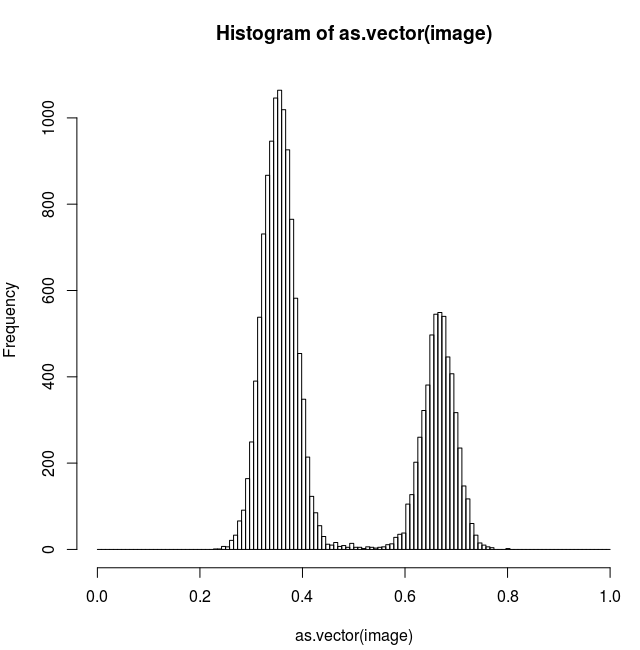
\includegraphics[scale=0.25]{image/128.png}
	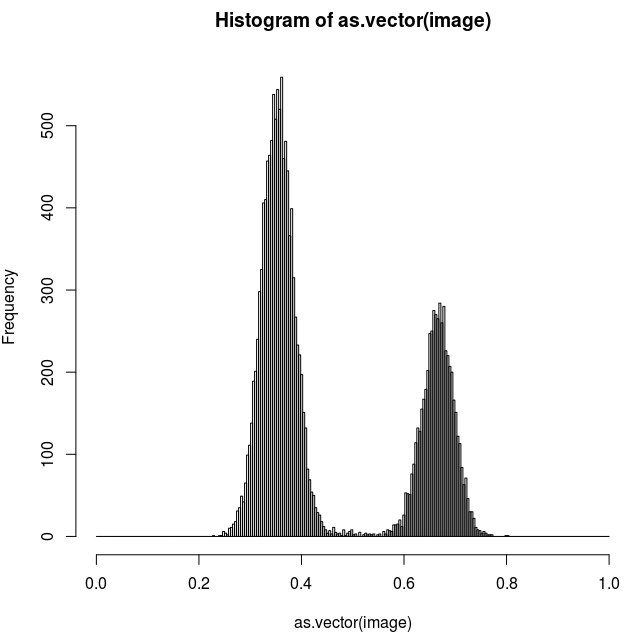
\includegraphics[scale=0.25]{image/256.png}
	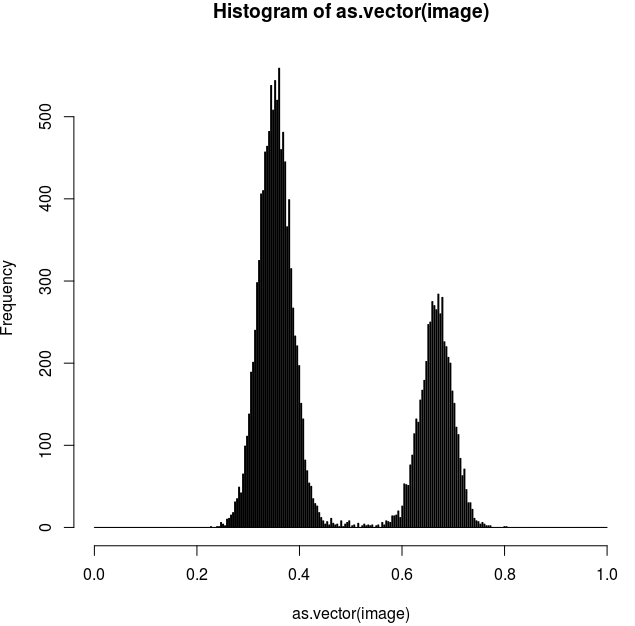
\includegraphics[scale=0.25]{image/512.png}
\end{figure}

Dans les images ci-dessus avec comme nbins respectivement égal  à 128, 256, 512 on remarque que 

\subsection*{Modifier la valeur de la variable seuil et commenter les résultats}

C'est le seuil qui permet de déterminer la binarisation. Imaginons que l'on ait 256 valeurs de gris. Si l'on met un seuil de 0.5 les niveaux de gris supérieurs à 256*seuil seront en noir et ceux inférieurs en blanc.

\begin{figure}[!ht]
	\center
	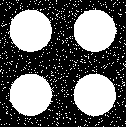
\includegraphics[scale=0.5]{image/04.png}
	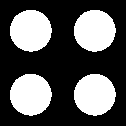
\includegraphics[scale=0.5]{image/05.png}
	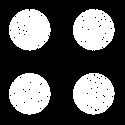
\includegraphics[scale=0.5]{image/06.png}
\end{figure}

Comme visible sur les images ci-dessus, ayant un seuil respectifs de 0.4, 0.5 et 0.6. Sur une image de seuil à 0 l'image binarisée sera blanche et sur une image de seuil 1, noir.

Si on se réfère aux histogrammes précédents le seuil correspond à l'axe des abscisses.

\newpage

%%%%%%%%%%%%%%%%%%%%%%%%%%%%%%%%%%%%%%%%%% PART 2
%%%%%%%%%%%%%%%%%%%%%%%%%%%%%%%%%%%%%%%%%%%%%%%%%
%%%%%%%%%%%%%%%%%%%%%%%%%%%%%%%%%%%%%%%%%%%%%%%%%
\section*{Histogramme des niveaux de gris}

\subsection*{Image 0}
\begin{figure}[!ht]
	\center
	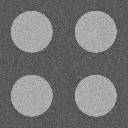
\includegraphics[scale=0.5]{../rdf-2-classes-texture-0.png}
	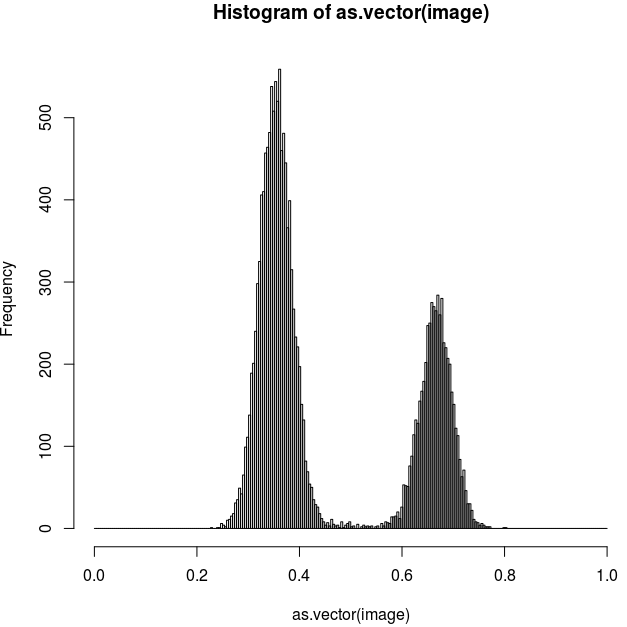
\includegraphics[scale=0.3]{image/text0.png}
	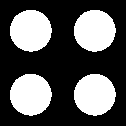
\includegraphics[scale=0.5]{image/text01.png}
\end{figure}

Pour l'image de gauche qui correspond à l'image des questions précédentes, on voit clairement sur l'histogramme que ca valeur de seuil optimale se trouve entre 0.4 et 0.6 soit $\sim$0.5. L'image résultante de la binarisation (image de droite), montre que 0.5 correspond à une valeur correcte.

\subsection*{Image 1}
\begin{figure}[!ht]
	\center
	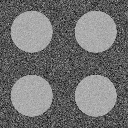
\includegraphics[scale=0.5]{../rdf-2-classes-texture-1.png}
	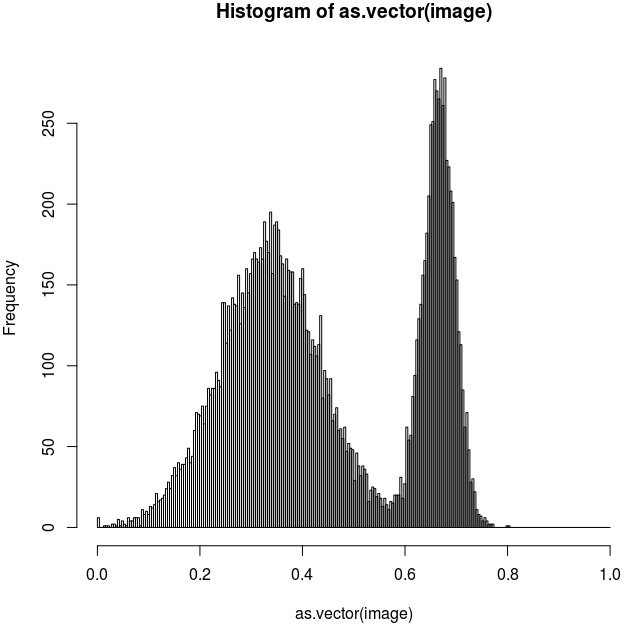
\includegraphics[scale=0.3]{image/text1.png}
	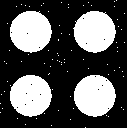
\includegraphics[scale=0.5]{image/text11.png}
\end{figure}

Pour cette image il est très compliqué d'avoir une binarisation parfaite à cause du bruit sur l'image. L'histogramme montre que, entre 0.5 et 0.6 c'est le meilleur seuil pour la binarisation. La valeur qui nous permet d'obtenir des cookies parfaitement blanc est $\sim$0.58, cependant le fond contient quelques pixels blanc.

\newpage

\subsection*{Image 2}
\begin{figure}[!ht]
	\center
	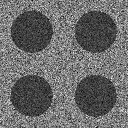
\includegraphics[scale=0.5]{../rdf-2-classes-texture-2.png}
	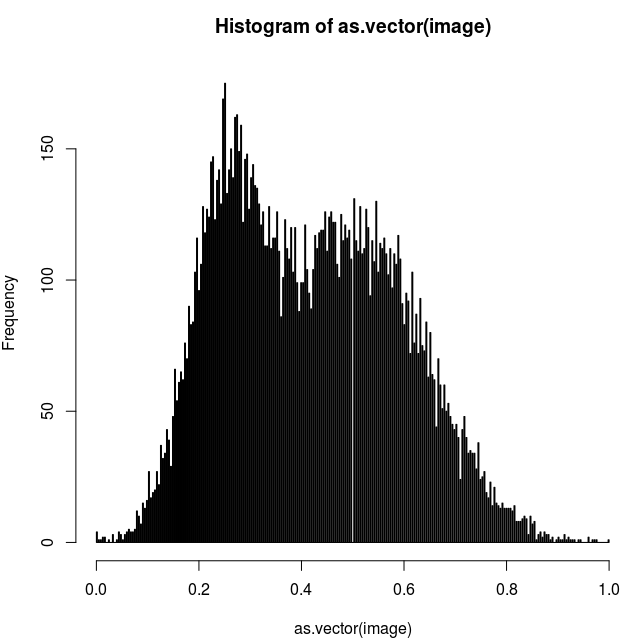
\includegraphics[scale=0.3]{image/text2.png}
	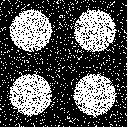
\includegraphics[scale=0.5]{image/text21.png}
\end{figure}

Pour cette image il est encore plus compliqué que précédemment d'avoir une binarisation parfaite à cause du bruit. L'histogramme montre une chute du nombre de niveau de gris à $\sim$0.31 nous avons donc choisis cette valeur de seuil et c'est cette valeur qui nous donne la meilleur distinction pour reconnaître visuellement les cookies. Le fond est cette fois constitué de pixels noir et de blanc.

\subsection*{Image 3}
\begin{figure}[!ht]
	\center
	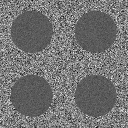
\includegraphics[scale=0.5]{../rdf-2-classes-texture-3.png}
	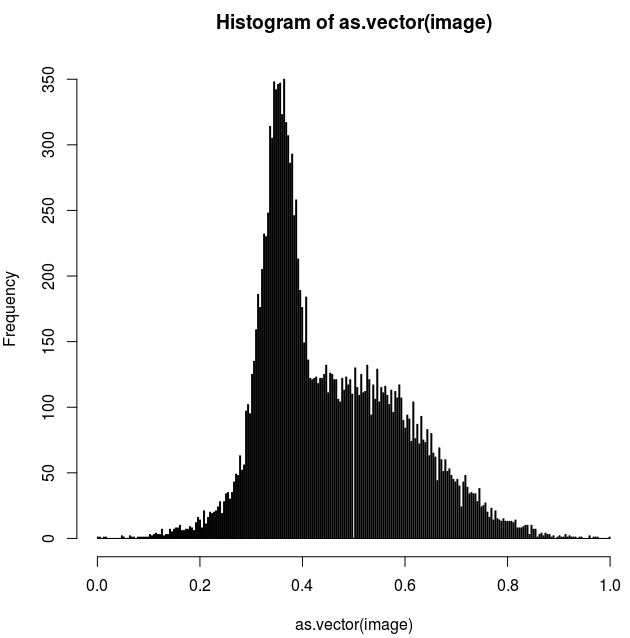
\includegraphics[scale=0.3]{image/text3.png}
	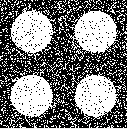
\includegraphics[scale=0.5]{image/text31.png}
\end{figure}

Pour cette image il est encore plus compliqué que précédemment d'avoir une binarisation parfaite à cause du bruit. L'histogramme montre un vide de gris à $\sim$0.4 nous avons donc choisis cette valeur de seuil et c'est cette valeur qui nous donne la meilleur distinction pour reconnaître visuellement les cookies. Le fond est cette fois constitué de pixels noir et de blanc.

\newpage 

\subsection*{Image 4}
\begin{figure}[!ht]
	\center
	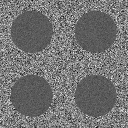
\includegraphics[scale=0.5]{../rdf-2-classes-texture-3.png}
	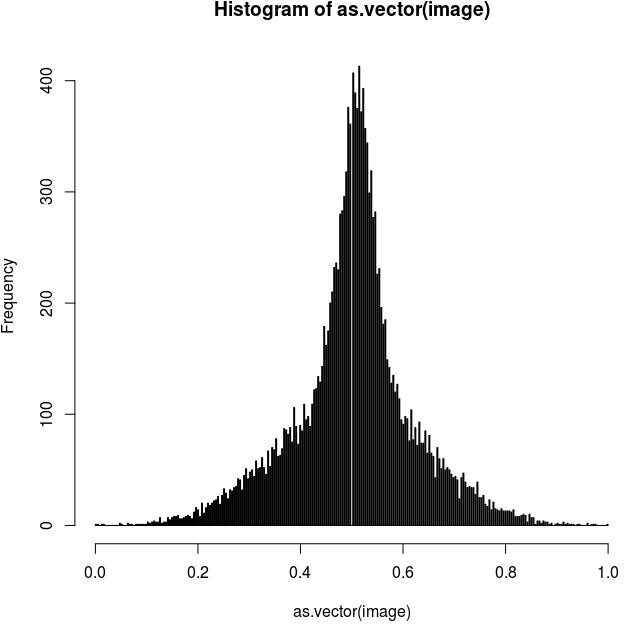
\includegraphics[scale=0.3]{image/text4.png}
	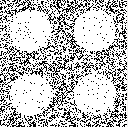
\includegraphics[scale=0.5]{image/text41.png}
\end{figure}


En observant l'histogramme il est difficile de déterminer quel sera la valeur du seuil. En essayant plusieurs valeur le seuil $\sim$0.45 nous permet de distinguer les cookies. Les niveaux de gris proches les uns des autres et le bruit augmente considérablement la difficulté d'obtenir une binarisation permettant de distinguer facielement les éléments voulus de l'image.

\subsection*{Pour chacune des images, comparer le résultat de votre binarisation avec l'image de référence et calculer le pourcentage de pixels pour lesquels la segmentation est erronée}

\begin{figure}[!ht]
	\center
	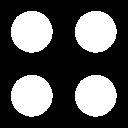
\includegraphics[scale=0.3]{../rdf-masque-ronds.png}
	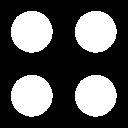
\includegraphics[scale=0.3]{../rdf-masque-ronds.png}
	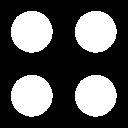
\includegraphics[scale=0.3]{../rdf-masque-ronds.png}
	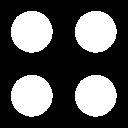
\includegraphics[scale=0.3]{../rdf-masque-ronds.png}
	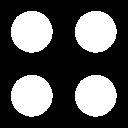
\includegraphics[scale=0.3]{../rdf-masque-ronds.png}
	\center
	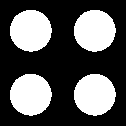
\includegraphics[scale=0.3]{image/text01.png}
	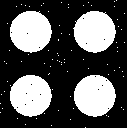
\includegraphics[scale=0.3]{image/text11.png}
	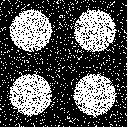
\includegraphics[scale=0.3]{image/text21.png}
	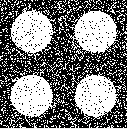
\includegraphics[scale=0.3]{image/text31.png}
	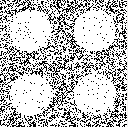
\includegraphics[scale=0.3]{image/text41.png}
	\center
	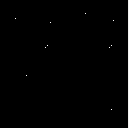
\includegraphics[scale=0.3]{image/diff0.png}
	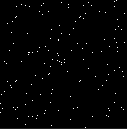
\includegraphics[scale=0.3]{image/diff1.png}
	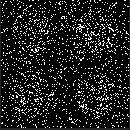
\includegraphics[scale=0.3]{image/diff2.png}
	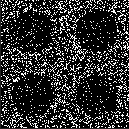
\includegraphics[scale=0.3]{image/diff3.png}
	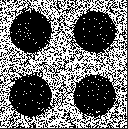
\includegraphics[scale=0.3]{image/diff4.png}
\end{figure}

Nous avons exprimé la différence sur la dernière ligne. On peux constater que sur la dernière image la différence est similaire à l'image que l'on obtient. Ceci est dûe à la proximitée des niveaux de gris, comme on l'avait constaté avec l'histogramme.

On en conclus donc que le bruit ainsi que la concentration des niveaux de gris (comme la dernière image) ne permet pas de binariser toute les images uniquement par leurs niveaux de gris et nous l'avons démontré avec la dernière image.

\begin{center}
\begin{longtable}[c]{|p{0.4\linewidth}| p{0.6\linewidth}|} 

	\hline
		\multicolumn{2}{|c|}{Différence de pixels} \\ \hline
	Image 0	&	(19/16384)*100 = 0.115\%\\ \hline
	Image 1	&	(145/16384)*100 = 0.885\% \\ \hline
	Image 2	&	(2097/16384)*100 = 12.799\\ \hline
	Image 3	&	(2994/16384)*100 = 18.273\%\\ \hline
	Image 4	&	(9206/16384)*100 = 56.188\%\\ \hline
	
\end{longtable}
\end{center}


%%%%%%%%%%%%%%%%%%%%%%%%%%%%%%%%%%%%%%%%%% PART 3
%%%%%%%%%%%%%%%%%%%%%%%%%%%%%%%%%%%%%%%%%%%%%%%%%
%%%%%%%%%%%%%%%%%%%%%%%%%%%%%%%%%%%%%%%%%%%%%%%%%
\section*{Histogramme des niveaux de texture}

\subsection*{Expliquer comment la fonction rdfTextureEcartType détermine le niveau de texture pour chaque pixel de l'image}

La fonction rdfTextureEcartType va dans un premier temps calculer le carré de l'image moin sa moyenne. Pour calculer sa moyenne il fait appel à la fonction rdfMoyenneImage qui calcule la matrice nécessaire pour déterminer la zone qui sera considérer autour de premier pixel. Une fois le contour calculé, la fonction filter est appelée pour appliquer le masque. Filter2 permet d'appliquer des filtres comme des flous, des détections de contours ...
Ensuite on calcule l'écart type et on normalise.

\subsection*{Comment fixe-t-on la dimension du voisinage de calcul grâce à l'argument taille passé à la fonction ?}

Comme dit précédemment le voisinage est calculé dans rdfMoyenneImage. La taille correspond au nombre de pixels voisines que l'on doit prendre en considération. Ensuite on calcul la dimension de la matrice pour déterminer l'ensemble de pixel. 1 de pixel donne 2*1+1, on obtient une matrice de dimension 3*3.

\subsection*{Pourquoi l'image écart-type est-elle normalisée ?}

Elle est normalisée car l'écart type calcul des valeurs qui sont supérieur aux valeurs de la matrice de base. Donc on normalise pour fournir des valeurs correspondantes aux valeurs de la matrice de base.

\newpage

\subsection*{ Calculer l'histogramme de chacune de ces images de niveau de texture et en déduire le seuil qui permet de la binariser au mieux}

\begin{figure}[htp]
  \centering
  \caption{Histogrammes}

  \subfloat[Histogramme 0]{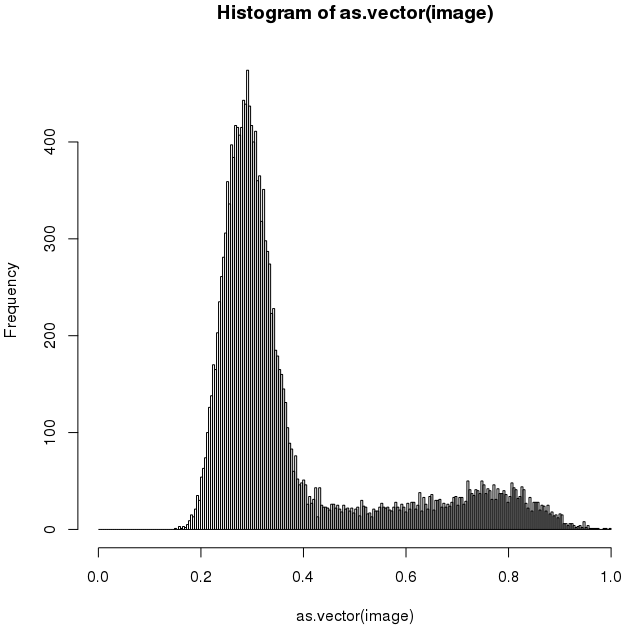
\includegraphics[scale=0.28]{image/p30.png}}
  \subfloat[Histogramme 1]{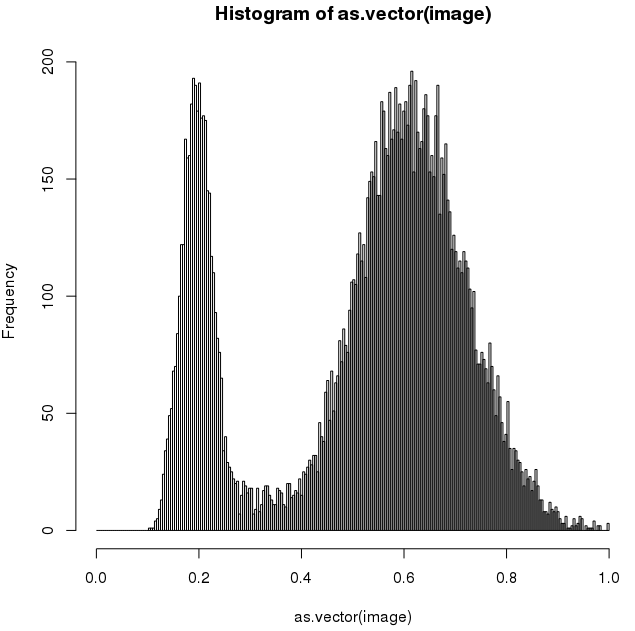
\includegraphics[scale=0.28]{image/p31.png}}
  \subfloat[Histogramme 2]{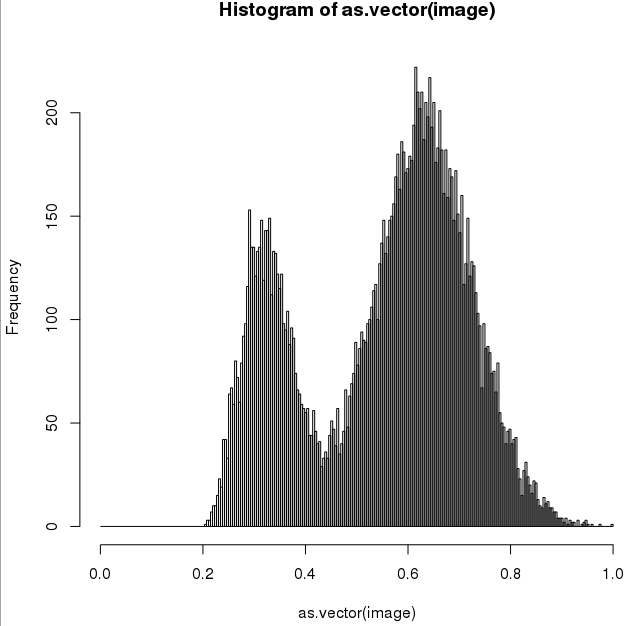
\includegraphics[scale=0.28]{image/p32.png}}
  \\
  \subfloat[Histogramme 3]{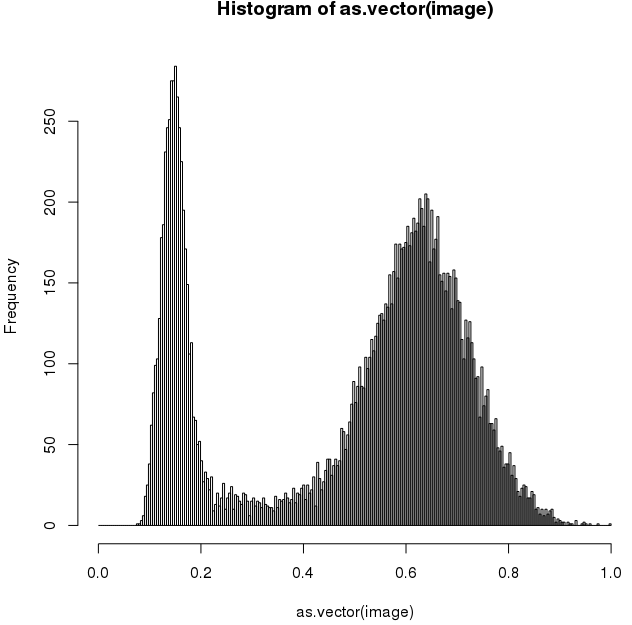
\includegraphics[scale=0.28]{image/p33.png}}
  \subfloat[Histogramme 4]{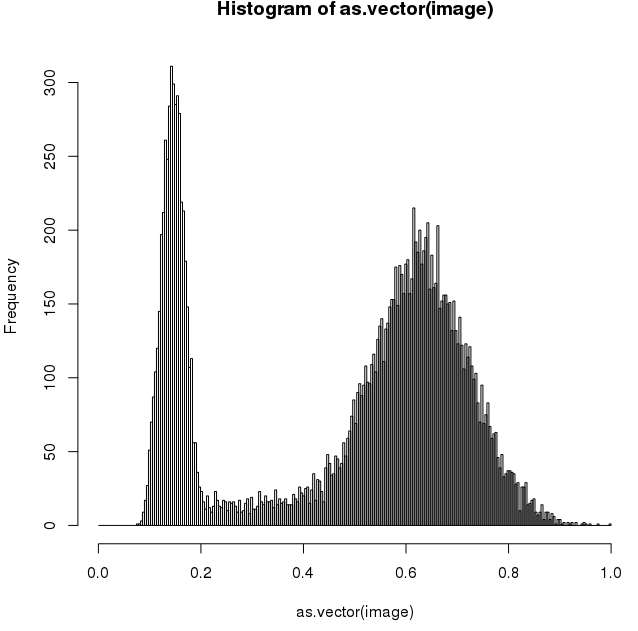
\includegraphics[scale=0.28]{image/p34.png}}

\begin{center}
\begin{longtable}[c]{|p{0.4\linewidth}| p{0.6\linewidth}|} 

	\hline
		\multicolumn{2}{|c|}{Seuil trouvé} \\ \hline
	Histogramme 0	&	 0.45\\ \hline
	Histogramme 1	&	 0.3\\ \hline
	Histogramme 2	&	 0.43\\	 \hline
	Histogramme 3	&	 0.35\\ \hline
	Histogramme 4	&	 0.3\\ \hline
	
\end{longtable}
\end{center}
\end{figure}

\newpage

\subsection*{En utilisant l'image de référence, calculer également le pourcentage de pixels mal segmentés dans chaque cas}

\begin{figure}[htp]
  \centering
	
\includegraphics[scale=0.3]{image/p3b0.png}
	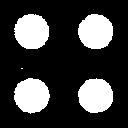
\includegraphics[scale=0.3]{image/p3b1.png}
	
\includegraphics[scale=0.3]{image/p3b2.png}
	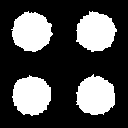
\includegraphics[scale=0.3]{image/p3b3.png}
	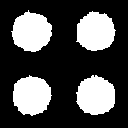
\includegraphics[scale=0.3]{image/p3b4.png}

\begin{center}
\begin{longtable}[c]{|p{0.4\linewidth}| p{0.6\linewidth}|} 

	\hline
		\multicolumn{2}{|c|}{Pourcentage de pixels mal segmentés} \\ \hline
	Image 0	&	 34.45\% \\ \hline
	Image 1	&	 9.8\% \\ \hline
	Image 2	&	 6.72\% \\	 \hline
	Image 3	&	 3.9\% \\ \hline
	Image 4	&	 4.06\% \\ \hline
	
\end{longtable}
\end{center}
\end{figure}

En observant les résultats nous obtenons des images certes, plus nettes malgrès le bruit en utilisant le niveau de  texture. Cependant sur des images qui à la base n'ont pas de bruit, le niveau de texture crée du bruit. L'image 0 est très différente de celle voulue. Nous pouvons donc conclure que le de niveau de texture ne peut être le seul attribut. Combiner plusieurs attributs est donc essentiel pour obtenir une binarisation proche de la perfection.

\newpage

%%%%%%%%%%%%%%%%%%%%%%%%%%%%%%%%%%%%%%%%%% PART 4
%%%%%%%%%%%%%%%%%%%%%%%%%%%%%%%%%%%%%%%%%%%%%%%%%
%%%%%%%%%%%%%%%%%%%%%%%%%%%%%%%%%%%%%%%%%%%%%%%%%

\section*{Histogramme conjoint}

\subsection*{Analyser le code de la fonction rdfCalculeHistogramme2D qui permet de calculer l'histogramme conjoint des deux attributs, en vous référant à la documentation de R pour les fonctions findInterval et table}

\begin{lstlisting}
rdfCalculeHistogramme2D <- function (image1, bins1, image2, bins2) {
  indices1 = findInterval (image1, seq (0, 1, 1 / bins1))
  indices2 = findInterval (image2, seq (0, 1, 1 / bins2))
  counts <- table (indices1, indices2)
  liste <- as.data.frame (counts)
  h2d <- array (0, c (bins1, bins2))
  h2d[cbind (liste[,1], liste[,2])] <- liste[,3]
  h2d <- log (1 + h2d)
  as.Image (h2d / max (h2d))
}
\end{lstlisting}

Dans un premier temps, la fonction va faire findInterval sur les 2 images. FindInterval permet de trouver l'interval entre les valeurs de la matrice x et y. Table ensuite va créer une matrice de 256x256 dans laquel il va comptabiliser le nombre d'occurence des valeurs de niveaux de gris.
Ensuite l'histogramme est créé.

\subsection*{Pour chacune des 5 images présentant les quatre ronds avec différentes variantes de texture, déterminer les histogrammes conjoints avec le niveau de gris et le niveau de texture comme attributs des pixels}

\begin{figure}[htp]
  \centering
	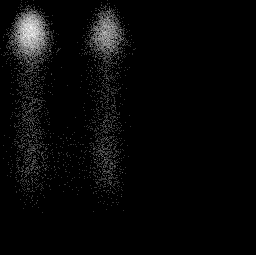
\includegraphics[scale=0.35]{image/hd0.png}
	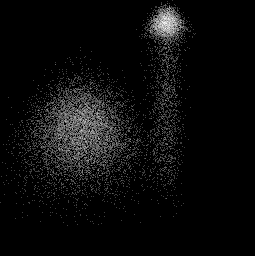
\includegraphics[scale=0.35]{image/hd1.png}
	\includegraphics[scale=0.35]{image/hd2.png}
	\includegraphics[scale=0.35]{image/hd3.png}
	\includegraphics[scale=0.35]{image/hd4.png}
\end{figure}

\subsection*{Sur chacun des histogrammes 2D, déterminer approximativement la droite qui sépare au mieux les deux régions correspondant: 1) au fond de l'image; 2) aux 4 disques}

\begin{figure}[htp]
  \centering
	\includegraphics[scale=0.35]{image/hd01.png}
	\includegraphics[scale=0.35]{image/hd11.png}
	\includegraphics[scale=0.35]{image/hd21.png}
	\includegraphics[scale=0.35]{image/hd31.png}
	\includegraphics[scale=0.35]{image/hd41.png}
\end{figure}

Il semble logique qu'une binarisation utilisant les deux méthodes donne des images binaires plus proche d'une image parfaite. Le pourcentage de pixel mal segmenté sera donc également diminué.

\section*{Conclusion}

Pour conclure, nous avons vu deux méthodes pour binariser. La méthode en utilisant les niveaux de gris, si inférieur au seuil donné alors 0 sinon 1. Dans l'autre méthode on à appliqué un filtre qui fait la moyenne des pixels voisins au pixel traité, cela correspond à un flou. Chacune de ces deux méthodes nous a fournit une binarisation des images. L'une d'entre elle fonctionnait quand le bruit n'était pas présent et l'autre fonctionnait parfaitement sur des images bruitées. Nous supposons que utiliser le classifieur linéaire va utiliser ces deux méthode pour une seule et unique binarisation pour obtenir une image binarisé se rapprochant au  mieux d'une image binaire parfaite. 

L'idée pouvant résulter de ces expériences est, si appliquer 2 attributs peut nous permettre d'obtenir une image proche de la perfection (en terme de binarisation), est-ce que appliquer une infinitée d'attributs nous permettra d'obtenir une image binaire parfaite ? C'est ce que nous pouvons imaginer et ce qui semble cohérent.


\end{document}
